\documentclass[12pt]{article}
\usepackage[OT1]{fontenc}
\usepackage[utf8]{inputenc}
\usepackage{kpfonts}
\usepackage{graphicx}
\usepackage[dvipsnames]{xcolor}
\usepackage{amsthm}
\usepackage[margin=1.25in]{geometry}
\usepackage[sf,bf,small,raggedright,compact]{titlesec}
\usepackage[capitalize]{cleveref}
\usepackage{paralist}



\newcommand{\pref}[1]{(P\ref{#1})}
\setlength{\parskip}{1ex}

\newtheorem{thm}{Theorem}
\newtheorem{obs}{Observation}
\newtheorem{lem}{Lemma}

\DeclareMathOperator{\dist}{d}
\DeclareMathOperator{\pack}{pack}
\DeclareMathOperator{\hit}{hit}

\newcommand{\defin}[1]{\emph{\textcolor{Maroon}{#1}}}

\newcommand{\pat}[1]{[\textcolor{red}{#1}]}

\title{Connected Dominating Sets in Triangulations}
\author{Prosenjit Bose \and Vida Dujmović \and Hussein Houdrouge \and Pat Morin \and Saeed Odak \and Anyone Else?}
\date{October 2023}



\begin{document}

\maketitle

% \begin{abstract}
%   We show that every $n$ vertex triangulation $G$ has a spanning tree with at least $n/2\pm{?}$ leaves.  This improves the previous best bound of $2n/5\pm {?}$, due to Kleitman and West (1991). \pat{Is this true? I only find $n/3$.}
% \end{abstract}


\section{Introduction}

A set $X$ of vertices in a graph $G$ is a \defin{dominating set} if each vertex of $G$ is in $X$ or adjacent to a vertex in $X$.  A dominating set $X$ of $G$ is \defin{connected} if the induced graph $G[X]$ is connected.

% Observe that, for any connected dominating set $X$, $G$ has a spanning-tree in which all vertices in $V(G)\setminus X$ are leaves.  Similarly, by removing the leaves of any spanning tree of $G$ we obtain a tree whose vertex set is a connected dominating set of $G$.
%  Therefore, an $n$-vertex graph $G$ has a connected dominating set of size $q$ if and only if $G$ has a spanning tree with at least $n-q$ leaves.

The main result in this paper is the following:

\begin{thm}\label{main_result2}
  For any $n\ge 4$, any $n$-vertex triangulation $G$ has a connected dominating set of size at most $10n/19 + O(1)$.
\end{thm}

\subsection{Related Work}

Dominating sets in graphs is an enormous field of research, with several books  devoted to the topic \cite{haynes.hedetniemi.ea:domination,haynes.hedetniemi.ea:topics}.

\pat{Expand.  Explain how Kleitman-West result gives $3n/4$.  Explain how Matheson-Tarjan gives $2n/3$.}


% \begin{thm}\label{main_result}
%   For any $n\ge 4$, any $n$-vertex triangulation $G$ has a connected dominating set of size at most $4n/7 + O(1)$.
% \end{thm}


\section{The Proofs}

For a graph $G$, let $|G|=|V(G)|$ denote the number of vertices of $G$.  A \defin{bridge} in a graph $G$ is an edge $e$ of $G$ such that $G-e$ has more connected components than $G$.  A \defin{plane graph} is a graph equipped with a non-crossing embedding in $\mathbb{R}^2$.  A plane graph is \defin{outerplane} if all its vertices appear on the outer face.  A \defin{triangle} is a cycle of length $3$. A \defin{near-triangulation} is a plane graph whose outer face is bounded by a cycle and whose inner faces are all bounded by triangles.  A \defin{generalized near-triangulation} is a plane graph whose inner faces are bounded by triangles.


For a plane graph $H$, we use the notation $B(H)$ to denote the vertex set of the outer face of $H$ and define $I(H):=V(H)\setminus B(H)$.  The vertices in $B(H)$ are \defin{boundary vertices} of $H$ and the vertices in $I(G)$ are \defin{inner vertices} of $H$. For any vertex $v$ of $H$, the \defin{inner neighbourhood} of $v$ in $H$ is defined as $N_H^+(v):=N_H(v)\cap I(H)$, the vertices in $N^+_H(v)$ are \defin{inner neighbours} of $v$ in $H$, and $\deg^+_H(v)=|N^+_H(v)|$ is the \defin{inner degree} of $v$ in $H$.

Let $G$ be a triangulation.  Our procedure for constructing a connected dominating set $X$ begins with an incremental phase that eats away at the triangulation $G$ ``from the outside.'' The process of constructing $X$ is captured by the following definition:   A vertex subset $X\subseteq V(G)$ is \defin{outer-domatic} if it can be partitioned into non-empty subsets $\Delta_0,\Delta_1,\ldots,\Delta_{r-1}$ such that
\begin{compactenum}[(P1)]
    \item $\Delta_0\subseteq B(G)$; \label{outer_face}
    \item $\Delta_i\subseteq B(G-(\bigcup_{j=0}^{i-1}\Delta_j))$ for each $i\in\{1,\ldots,r-1\}$; and \label{incremental}
    \item $G-(\bigcup_{j=0}^{r-1}\Delta_j)$ is outerplanar. \label{outerplanar}
\end{compactenum}

\begin{lem}\label{outer_domatic}
    Let $G$ be a triangulation.  Then any outer-domatic $X\subseteq V(G)$ is a connected dominating set of $G$.
\end{lem}

\begin{proof}
  Suppose $X$ is outer-domatic and let $\Delta_0,\ldots,\Delta_r$ be the corresponding partition of $X$.  For each $i\in\{1,\ldots,r\}$, let $X_i:=\bigcup_{j=0}^{i-1} \Delta_i$.  First observe that, since $\Delta_0\subseteq B(G)$ is non-empty, $X_i$ contains at least one vertex of $B(G)$, for each $i\in\{1,\ldots,r\}$. We claim that
  \begin{compactenum}[(P1)]\setcounter{enumi}{3}
    \item each vertex in $B(G-X_{i-1})$ is adjacent to some vertex in $X_{i-1}$, for each $i\in\{2,\ldots,r\}$. \label{adjacent}
  \end{compactenum}
  Indeed, for any $i\in\{2,\ldots,r\}$ and any vertex $v\in B(G-X_{i-1})$ is either in $B(G)$ or adjacent to a vertex in $X_{i-1}$. Even in the former case $v$ is adjacent to a vertex in $X_1=\Delta_0\subseteq X_{i-1}$, because because $G[B(G)]$ is a clique.

  We now prove, by induction on $i$, that $G[X_i]$ is connected, for each $i\in\{1,\ldots,r\}$.
  The fact that $G[B(G)]$ is a clique and \pref{outer_face} implies that $G[X_1]=G[\Delta_0]$ is connected. For each $i\in\{2,\ldots,r\}$, the assumption that $G[X_{i-1}]$ is connected, \pref{incremental}, and \pref{adjacent} then imply that $G[X_i]=G[X_{i-1}\cup\Delta_{i-1}]$ is connected.

  In particular $G[X_r]=G[X]$ is connected.  Finally, \pref{adjacent}, with $i=r$ and \pref{outerplanar} implies that $N_G(X_r)=B(G-X_r)=V(G-X_r)$, so $X_r=X$ is a dominating set of $G$.
\end{proof}

We will present two algorithms that grow a connected dominating in small batches $\Delta_0,\Delta_1,\ldots,\Delta_{r-2}$ that result in a sequence of sets $X_1,\ldots,X_{r-1}$ where $X_{i}=\bigcup_{j=0}^{i-1}\Delta_j$.  However, each of these algorithms is unable to continue once they reach a point where each vertex in $B(G-X_i)$ has inner-degree at most $1$ in $G-X_i$.  We begin by studying the graphs that cause this to happen.

\subsection{Critical Graphs}

A generalized near-triangulation $H$ is \defin{critical} if $\deg^+_H(v)\le 1$ for each $v\in B(H)$.


\begin{lem}\label{base_case}
    Let $H$ be critical generalized near-triangulation. Then $|B(H)|\ge 3|I(H)|$ and there exists $\Delta\subseteq B(H)$ of size at most $|I(H)|$ that dominates $I(H)$.
\end{lem}

\begin{proof}
  Let $B:=B(H)$ and $I:=I(H)$.  If $I$ is empty then the result is trivially true, by taking $X:=\emptyset$, so we now assume that $I$ is non-empty.  By definition, the graph $H[B]$ is outerplanar.  Say that an inner face of $H[B]$ is \defin{marked} if it contains an inner vertex of $H$.  Consider some marked face $f$ of $H[B]$.  This face is marked because it contains at least one vertex in $I$.  Since $G$ is a triangulation, there is an edge $vx$ in $G$ with $v\in B$ on the boundary of $f$ and $x\in I$ in the interior of $f$.  The vertex $v$ is incident to an edge $vw$ on the boundary of $f$. By the same reasoning $G$ contains an edge $wx'$ with $x'\in I$ in the interior of $f$.  Therefore $\deg^+_H(v),\deg^+_H(w)\ge 1$ and since $H$ is critical, $\deg^+H(v)=\deg^+_H(w)=1$.  Since $G$ is a triangulation the triangle $vwx$ is a face of $G$ and the triangulation $vwx'$ is a face of $G$.  Since $\deg^+H(v)=\deg^+_H(w)=1$, $x=x'$.  We can make this argument for each edge of $f$ to conclude that $f$ contains exactly one vertex $x_f$ of $I$ and $x_f$ is adjacent to each vertex of $f$.  Thus, $H$ is formed from an outerplanar graph $H[B]$ by adding $|I|$ stars, one in the interior of each marked face of $H[B]$.  Furthermore, since $\deg_H^+(v)=1$ for each $v\in B$, each vertex of $H[B]$ is on the boundary of exactly one marked face.

    \begin{figure}
        \begin{center}
            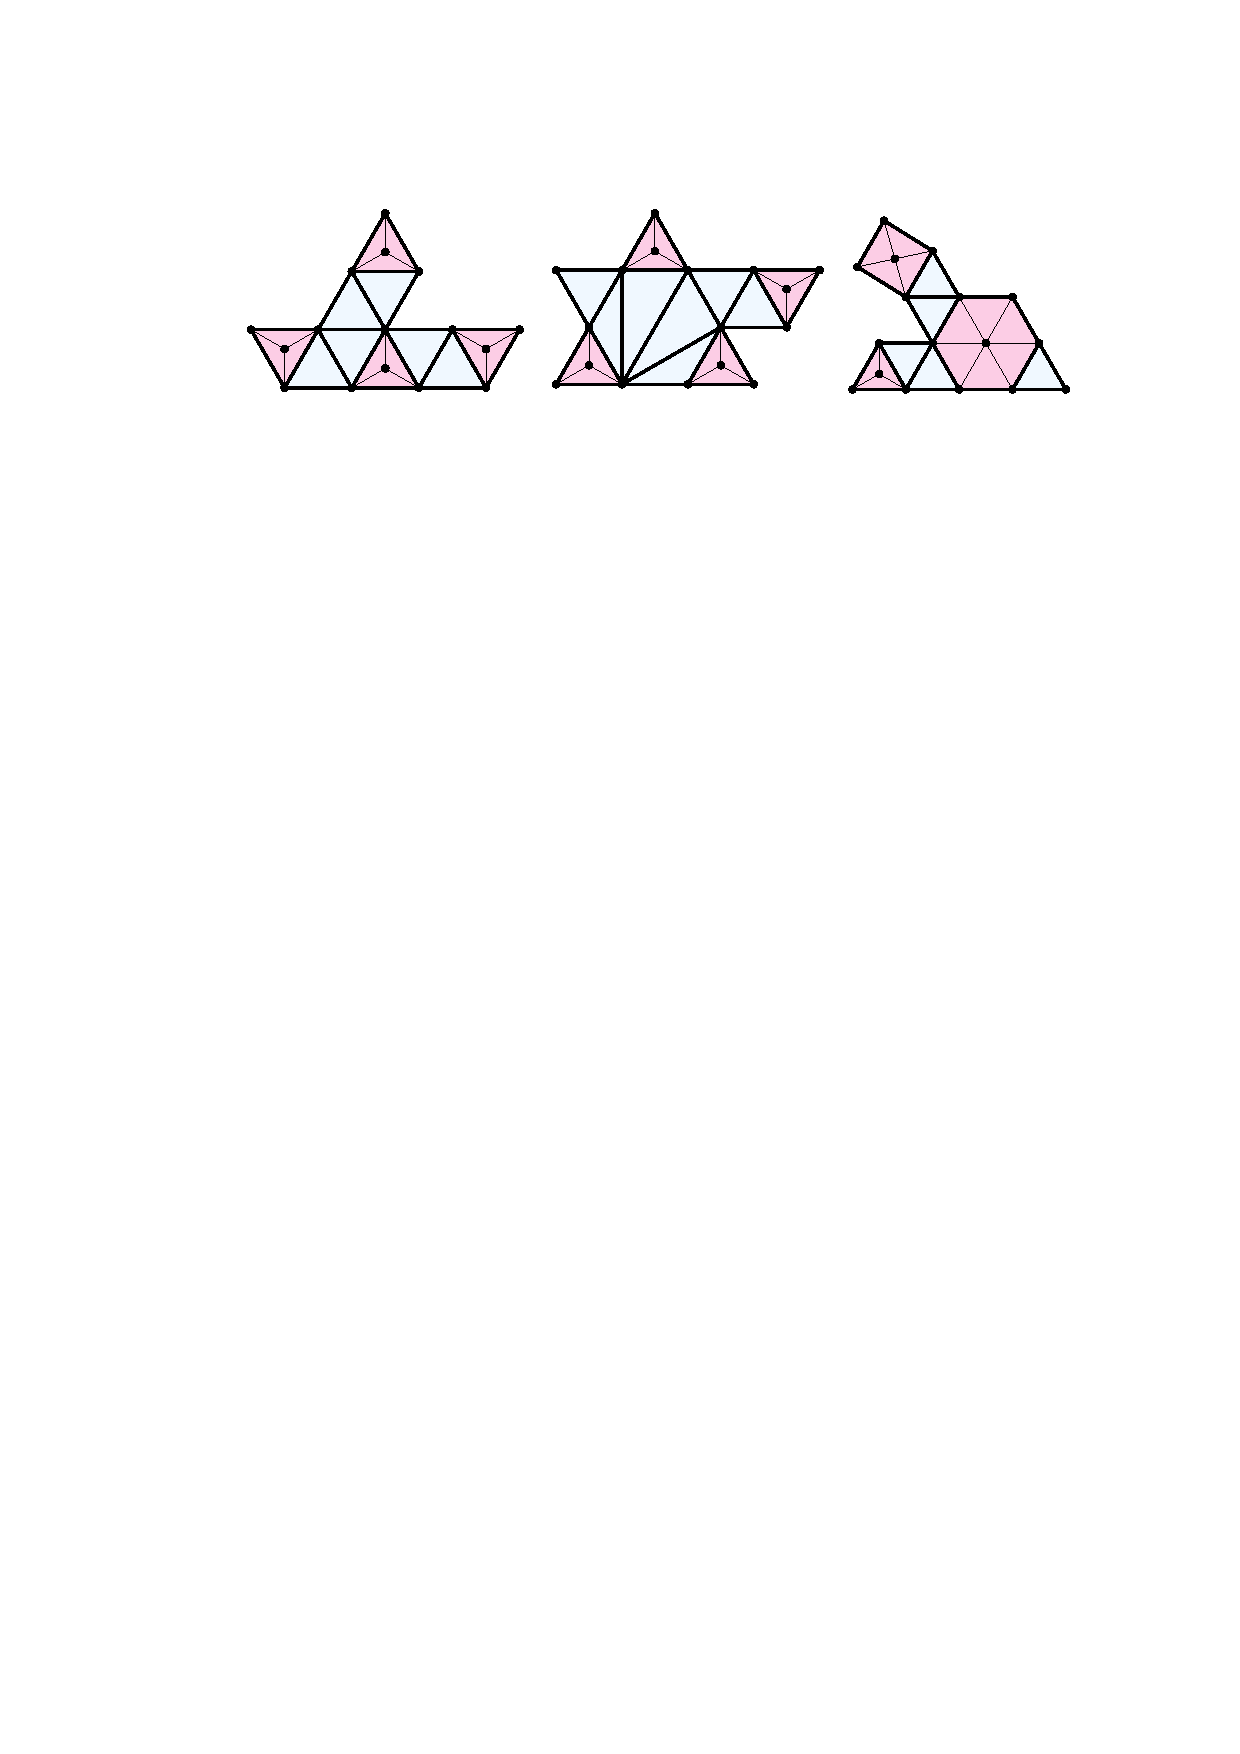
\includegraphics[page=1]{figs/critical} \\
            % \includegraphics[page=2]{figs/critical} \\
        \end{center}
        \caption{Some critical graphs \pat{Add some examples where $H[B(H)]$ has some non-triangular faces}}
        \label{critical_fig}
    \end{figure}

  Consider the graph $H'$ obtained by adding edges to the inner faces of $H[B]$ so that each inner face is a triangle. For each marked face $f$ of $H[B]$, select one triangular face $t_f$ of $H'$ that is contained in $f$ and \defin{mark} $t_f$.  Observe that the three vertices of $t_f$ are all adjacent, in $G$ to $x_f$.  Thus there is a bijection from the set of marked faces of $H[B]$ to the set of marked faces in $H'$ and both of these sets have size $|I|$.  Since each vertex in $B$ is on the boundary of at most one marked face of $H[B]$, each vertex in $B$ is on the boundary of at most one marked triangular face of $H'$.  Therefore, $|B| \ge 3|I|$ so $|H|=|B|+|I|\ge 4|I|$.  By choosing one vertex from each marked triangular face of $H'$ we obtain the desired set $\Delta$.
\end{proof}


We note that the implementation of $\textsc{SimpleGreedy}(G)$ is even simpler than the definition given above.  Nothing special needs to be done for the graph $G_{r-1}$.  Repeatedly selecting a vertex of maximum innner-degree and removing it will produce a dominating set of size exactly $|I_{r-1}|$.  Thus, $\textsc{SimpleGreedy}(G)$ has a simple linear time implementation.  In this implementation, each vertex $v$ stores a value $d_v$ which is initially set to $\deg_G(v)$.  For the three vertices on the outer face of $G$, $d_v$ is set to $\deg_G(v)-2$.  In general,





Besides the data structure used for representing the triangulation $G$, the most sophisticated data structure needed is a doubly-linked list which stores the vertices of $B(G_i)$ grouped by their inner-degree, with these groups ordered in decreasing order of inner-degree.  The algorithm chooses a vertex $v_i$ from the first group, adds all the neighbours of $v_i$ to $B_i$




\section{A Simple Algorithm}

% We will construct a sequence of vertex sets $\emptyset = X_0\subsetneq X_1\subsetneq\cdots\subsetneq X_r$ such that $G[X_i]$ is connected for each $i\in\{1,\ldots,r\}$ and $X_r$ dominates $G$.  Let $G_0:=G$, let $D_0:=B_0:=B(G_0)$, and let $I_0:=V(G_0-D_0)$. For each $i\in\{1,\ldots,r\}$, let $D_i:=N_G[X_i]$, let $I_i:=V(G-D_i)$, let $B_i:=N_G(I_i)$, let $\Delta_{i-1}:=X_{i}\setminus X_{i-1}$, and let $G_i:=G[I_i\cup B_i]$.


% In words, $D_i$ contains all the vertices that are dominated by $X_i$; $I_i$ contains the vertices that are not dominated by $X_i$; $B_i$ contains all the vertices on the boundary between $X_i$ and $I_i$ (each vertex in $B_i$ is adjacent to at least one vertex in $X_i$ and at least one vertex in $I_i$); and $\Delta_i$ is the set of vertices we add to $X_i$ to get $X_{i+1}$. These sets will obey the following conditions:
% \begin{compactenum}[(P1)]
%     \item $\Delta_i\subseteq B_i$, for each $i\in\{0,\ldots,r-1\}$;
%     \item $G_r$ is outerplane.
% \end{compactenum}

We start with the simplest imaginable greedy algorithm, that we call $\textsc{SimpleGreedy}(G)$, to choose $\Delta_0,\ldots,\Delta_{r-1}$.  Suppose we have already chosen $\Delta_0,\ldots,\Delta_{i-1}$ for some $i\ge 0$ and we now want to choose $\Delta_i$.  Let $X_i:=\bigcup_{j=0}^{i-1}\Delta_j$, let $G_i:=G-X_i$, and let $v_i$ be a vertex in $B(G_i)$ that maximizes $\deg^+_{G_i}(v_i)$.  During iteration $i\ge 0$, there are only two cases to consider:
\begin{compactenum}
    \item If $\deg^+_{G_i}(v_i)\ge 2$ then we set $\Delta_i\gets\{v_i\}$.
    \item If $\deg^+_{G_i}(v_i)\le 1$ for all $v\in G_i$ then $G_i$ is critical and this is the final step, so $r:=i+1$.  By \cref{base_case}, there exists $\Delta_i\subseteq B_i$ of size at most $|I_i|$ that dominates $I_i$. Then $X_r:=X_{r-1}+\Delta_{i}$ and we are done.
\end{compactenum}

\begin{thm}\label{simple_greedy}
  When applied to an $n$-vertex triangulation $G$,  $\textsc{SimpleGreedy}(G)$ produces a connected dominating set $X_r$ of size at most $(4n+6)/7$.
\end{thm}

\begin{proof}
By the choice of $\Delta_0,\ldots,\Delta_{r-1}$, $X_r$ is an outer-domatic subset of $V(G)$ so, by \cref{outer_domatic}, $X_r$ is a connected dominating set of $G$.  All that remains is to analyze the size of $X_r$.  For each $i\in\{1,\ldots,r\}$, let $D_i:=N_G(X_i)$ be the subset of $V(G)$ that is dominated by $X_i$, let $I_i:=V(G)\setminus D_i$ be the subset of $V(G)$ not dominated by $X_i$, and let $B_i:=N_G(I_i)$ be the vertices of $G$ that have at least one neighbour in each of $X_i$ and $I_i$.  We use the convention that $D_0:=B(G)$.

First observe that, for $i\in\{0,\ldots,r-2\}$, $|D_{i+1}|\ge |D_i|+\deg_{G_i}^+(v_i)$ since $D_{i+1}\supseteq D_i$ and $D_{i+1}$ contains the $\deg_{G_i}^+(v_i)$ inner neighbours of $v_i$ in $G_i$.  Therefore
\[
    |D_{r-1}| \ge |D_0| + \sum_{i=0}^{r-2} \deg_{G_i}^+(v_i) \ge 3 + \sum_{i=0}^{r-2} 2 =  2r+1 \enspace . \label{double_d}
\]
Since $D_{r-1}$ and $I_{r-1}$ partition $V(G)$,
\begin{equation}
  n = |D_{r-1}| + |I_{r-1}| \ge 2r+1 + |I_{r-1}|  \enspace . \label{c1}
\end{equation}
% so
% \begin{equation}
%     r\le \frac{n-|I_{r-1}|-1}{2}  \enspace .
% \end{equation}

Since $X_{r-1}$ and $B_{r-1}$ are disjoint and $D_{r-1}\supseteq B_{r-1}\cup X_{r-1}$, we have $|D_{r-1}|\ge |X_{r-1}| + |B_{r-1}|=r-1+|B_{r-1}|$.  Therefore,
\begin{equation}
    n = |D_{r-1}| + |I_{r-1}| \ge r-1 + |B_{r-1}| + |I_{r-1}| = r-1 + |B_{r-1}| + |I_{r-1}|
    \ge r - 1 + 4|I_{r-1}| \enspace , \label{c2}
\end{equation}
where the last inequality follows from \cref{base_case}.

The final dominating set $X_r$ has size $|X_r| = |X_{r-1}| + \Delta_{r-1} = r - 1 +|I_{r-1}|$, so the size of $|X_r|$ can be upper-bounded by maximizing $r+|I_{r-1}|$ subject to the constraints \cref{c1,c2}.  More precisely, the maximum size of $X_r$ is upper bounded by the maximum value of $x-1+y$ subject to the constraints
\begin{align*}
  x - 1 + 4y & \le n \\
  2x + y +1 & \le n
\end{align*}

% r\le (n+1-I_{r-1})/2$ and $r+4|I_{r-1}|\le n$.
This is an easy linear programming exercise and the maximum value of $X_{r}$ is obtained when $r=(3n-5)/7$ and $|I_{r-1}|=(n+3)/7$, which gives
$|X_r| \le (4n-9)/7$.
\end{proof}

\section{A Less Simple Algorithm}

Next we devise an algorithm that produces a smaller connected dominating set than what is guaranteed by $\textsc{SimpleGreedy}(G)$.  This involves a more careful analysis of the cases in which \textsc{SimpleGreedy} is forced to take a vertex $v_i$ with $\deg^+_{G_i}(v_i)=2$.  We begin by identifying unnecessary vertices and edges that can appear in the graphs $G_1,\ldots,G_{r-1}$ during the construction of $X$.   We say that a near-triangulation $H$ is \defin{dom-minimal} if
\begin{compactenum}[({DM}1)]
    \item $\deg^+_H(v)\ge 1$ for each $v\in B(H)$; and \label{bad_vertex}
    \item $vw$ is on the boundary of an inner face $vwx$ for some $x\not\in B(H)$, for each edge $vw\in G[B(H)]$. \label{bad_edge}
\end{compactenum}
We say that a generalized near-triangulation $H$ is \defin{dom-minimal} if each of its biconnected components are dom-minimal.

\begin{obs}
    Any dom-minimal generalized near-triangulation $H$ is bridgeless.
\end{obs}

\begin{proof}
   If $vw$ is a bridge in $H$ then both $v$ and $w$ are in $B(H)$.  Since $vw$ is a bridge in $H$, there is no inner face $vwx$ in $H$. Thus $H$ does not satisfy the second condition for dom-minimality.
\end{proof}

A subgraph $H'$ of a generalized near-triangulation $H$ is \defin{dom-preserving} if
\begin{compactenum}[({DP}1)]
  \item $B(H')\subseteq B(H)$;
  \item $N^+_{H'}(v)=N^+_H(v)$ for all $v\in B(H')$;
  \item $I(H')=I(H)$; and
  \item $N_{H'}(v)=N_H(v)$ for all $v\in I(H)$.
\end{compactenum}

\begin{obs}
  Let $H$ be a generalized near-triangulation, let $H'$ be a dom-preserving subgraph of $H$, and let $\Delta$ be a subset of $V(H)$ that dominates $I(H)$.  Then $\Delta\cap V(H')$ dominates $I(H)$.
\end{obs}

\begin{proof}
  Each vertex $v\in I(H')$ is adjacent to some vertex $w\in \Delta$.  Since $N_{H'}(v)=N_H(v)$, $w\in\Delta\cap V(H')$, so $v$ is dominated by $\Delta\cap V(H')$.  Since this is true for each $v\in I(H)=I(H')$, $\Delta\cap V(H')$ dominates $I(H)$.
\end{proof}

\begin{lem}\label{dom-minimal}
  For any generalized near-triangulation $H$, there exists a dom-preserving subgraph $H'$ of $H$ that is dom-minimal.
\end{lem}

\begin{proof}
  The proof is by induction on $|V(H)|+|E(H)|$.  If $H$ is already dom-minimal, then setting $H'=H$ satisfies the requirements of the lemma, so assume that $H$ is not dom-minimal.  It is straightforward to verify that the dom-preserving subgraph relationship is transitive, so if $H$ has a dom-preserving subgraph $H^*$ and $H^*$ has a dom-preserving subgraph $H'$ then $H'$ is a dom-preserving subgraph of $H$.  Therefore, it is sufficient to show the existence of a dom-preserving subgraph $H^*$ of $H$ with fewer edges or fewer vertices than $H$, and the inductive hypothesis provides the desired dom-minimal dom-preserving subgraph $H'$ of $H$.

  If $H$ contains a vertex $v\in B(H)$ with $\deg^+_H(v)=0$ then $H-v$ is a dom-preserving subgraph of $H$ with fewer vertices than $H$.  We now assume that $\deg^+_H(v)\ge 1$ for all $v\in B(H)$.

  Since $H$ is not dom-minimal then $H$ contains a biconnected component $C$ that is not dom-minimal.
  \begin{compactenum}
    \item If there exists an edge $vw$ on the outer face of $C$ that is not incident to any inner face $vwx$ with $x\in I(C)$ then $B(H-vw)=B(H)$ and $I(H-vw)=I(H)$, and $H-vw$ is a is dom-preserving subgraph of $H$ that has fewer edges than $H$.

    \item If there exists a vertex $v\in B(C)$ with $\deg^+_C(v)=0$ then $v$ is incident to an edge $vw$ that is on the outer face of $C$ and on the outer face of $H$. Since $\deg^+_C(v)=0$, $vw$ is not incident to any inner face $vwx$ with $x\in I(C)$ and we can proceed as in the previous case. \qedhere
  \end{compactenum}
\end{proof}

We say that a generalized near-triangulation $H$ is \defin{good} if
\begin{compactenum}[(G1)]
      \item $H$ is critical;
      \item there exists $v\in B(H)$ with $\deg^+_H(v)\ge 3$; or
      \item there exists distinct $v,w\in B(H)$ such that $\deg^+_H(v)=2$ and $N^+_H(w)\subseteq N^+_H(v)$.
\end{compactenum}

\begin{lem}\label{not_good}
  Let $H$ be a dom-minimal generalized near-triangulation.  Then \begin{compactenum}[(i)]
    \item $H$ is good or
    \item $B(H)$ contains a vertex $v$ with $\deg^+_H(v)=2$ such that $G-v$ is good.
  \end{compactenum}
\end{lem}

\begin{proof}
  Since $H$ is dom-minimal, each vertex in $B(H)$ has inner-degree greater than $0$.  If some vertex in $B(H)$ has inner-degree at least $3$ then $H$ is good and there is nothing to prove, so we may assume that each vertex in $B(H)$ has inner-degree $1$ or $2$.  Since $H$ is not critical, at least one vertex in $B(H)$ has inner-degree $2$.

  If $H$ is $2$-connected, let $C:=H$ and let $v_0$ be any vertex of $H$ with inner-degree $2$.
  If $H$ is not $2$-connected, then let $C$ be a biconnected component of $H$ that contains a single cut-vertex $v_0$ of $H$ (so $C$ is a leaf in the block-cut tree of $H$). Then $v_0$ is contained in a second biconnected component $C'\neq C$ of $H$. Since $H$ is dom-minimal, $\deg^+_{C}(v_0)\ge 1$ and $\deg^+_{C'}(v_0)\ge 1$, so $\deg^+_H(v)= 2$.

  Since $C$ is biconnected its outer face is bounded by a cycle $v_0,v_1,v_2,\ldots,v_{k-1}$.  From this point on, all subscripts on $v$ are taken modulo $k$.  If $\deg^+_C(v_1)=1$ then, since $H$ is dom-minimal, the edge $v_0v_1$ is on the boundary of an inner face $v_0v_1x$ with $x\in I(H)$.  Since $v_0$ is the only cut-vertex of $H$ in $C$, $N^+_H(v_1)=N^+_C(v_1)=\{x\}\subseteq N_H(v_0)$ and $\deg^+_H(v_0)=2$, so $H$ is good and there is nothing to prove.  We now assume that $\deg^+_C(v_1)=2$.  By the same reasoning, we may assume that $\deg^+_C(v_i)=2$ for each $i\in\{1,\ldots,k-1\}$.  (Otherwise, $N^+_H(v_i)\subseteq N^+_H(v_{i-1})$ and $\deg^+_H(v_{i-1})=2$ for some $i\in\{2,\ldots,k-1\}$ and $H$ is good.)

  To summarize, so far we know that some vertex $x\in I(H)$ is in $N^+_H(v_0)$, $N^+_H(v_1)$, and $N^+_H(v_{k-1})$.  If $k=3$ then, since $H$ is dom-minimal, $H$ contains a face $v_1v_{k-1}y$ with $y\in I(H)$.  Since $\deg^+_H(v_1)=\deg^+_H(v_{k-1})=2$, $y\neq x$ and $N^+_H(v_1)=N^+_H(v_2)=\{x,y\}$. Again, this implies that $H$ is good.

  If $k\ge 4$, then consider the vertex $v_2$. The edge $v_1v_2$ is on the boundary of a face $v_1v_2y$.  Since $\deg^+_H(v_1)=2$, $x\neq y$.  If $N^+_H(v_1)=N^+_H(v_2)=\{x,y\}$ then $v_1$ and $v_2$ satisfy (GM3), so $H$ is good.  Otherwise, consider the graph $H':=H-v_0$.  Then $\deg^+_{H'}(v_1)=1$, $\deg^+_{H'}(v_2)=2$, and $N_{H'}(v_1)\subseteq N_{H'}(v_2)$.   Therefore $G'$ is good, so $G$ contains a vertex $v=v_0$ of inner-degree $2$ such that $G-v$ is good.  This completes the proof.
\end{proof}


This gives variant of the $\textsc{SimpleGreedy}(G)$ that we call $\textsc{BetterGreedy}(G)$.  Suppose we have already chosen $\Delta_0,\ldots,\Delta_{i-1}$ for some $i\ge 0$ and we now want to choose $\Delta_i$.  Let $X_i:=\bigcup_{j=0}^{i-1}\Delta_j$, let $G_i$ be a dom-preserving subgraph of $G-X_i$ that is dom-minimal, and let $v_i$ be a vertex in $B(G_i)$ that maximizes $\deg^+_{G_i}(v_i)$.  During iteration $i\ge 0$, there are only two cases to consider:
\begin{compactenum}
    \item If $\deg^+_{G_i}(v_i)\ge 3$ then we set $\Delta_i\gets\{v_i\}$.
    \item If there exists distinct $v_i,w\in B(H)$ such that $\deg^+_H(v)=2$ and $N^+_H(w)\subseteq N^+_H(v)$ then set $\Delta_i:=\{v_i\}$.
    \item If $\deg^+_{G_i}(v_i)\le 1$ for all $v\in G_i$ then $G_i$ is critical and this is the final step, so $r:=i+1$.  By \cref{base_case}, there exists $\Delta_i\subseteq B_i$ of size at most $|I_i|$ that dominates $I_i$. Then $X_r:=X_{r-1}+\Delta_{i}$ and we are done.
    \item Otherwise, $G_i$ is not good.  By \cref{not_good}, $G$ contains a vertex $v_i$ such that $G-v_i$ is good.  Set $\Delta_i:=\{v_i\}$.
\end{compactenum}

\begin{thm}\label{better_greedy}
  When applied to an $n$-vertex triangulation $G$,  $\textsc{BetterGreedy}(G)$ produces a connected dominating set $X_r$ of size at most $10n/19\pm{?}$.
\end{thm}

\begin{proof}
  Let $x_2$ be the number of times $\textsc{BetterGreedy}(G)$ falls into Case~4.
  For each integer $t\ge 3$, let $x_t$ be the number of times $\textsc{BetterGreedy}(G)$ falls into case $1$ and chooses $v_i$ such that $\deg^+_{G_i}(v_i)=t$.  Let $z$ be the number of times $\textsc{BetterGreedy}(G)$ falls into Case~2.  From \cref{not_good}, we know that
  \begin{equation}
      x_2 \le \sum_{t\ge 3}x_t + z \enspace .
  \end{equation}
  The size of the dominated set $D_{r-1}$ is at least
  \[
    |D_{r-1}| \ge 3 + \sum_{t\ge 2}tx_t + 2z
  \]
  The size of the boundary $B_{r-1}$ is at most
  \begin{equation}
       |B_{r-1}| \le 3 + \sum_{t\ge 2} (t-1)x_t \\
  \end{equation}
  By definition,
  \[
     r-1 = |X_{r-1}| = \sum_{t\ge 2} x_t + z
  \]
  As in the previous proof, we combine these constraints with the constraints $n=|D_{r-1}|+|I_{r-1}|$,  $|D_{r-1}|\ge r-1+|B_{r-1}|$ and $|D_{r-1}|\ge r-1+3|I_{r-1}|$.

  Here is an approximation of this in Sage:
  \begin{verbatim}
p = MixedIntegerLinearProgram()
v = p.new_variable()
D, I, B, r, n, x2, x3, x4, x5, x12 = v["D"], v["I"], v["B"], v["r"], v["n"], v["x2"], v["x3"], v["x4"], v["x5"], v["x12"]
N = 1000000000
p.add_constraint(n <= N)
p.add_constraint(x2 >= 0)
p.add_constraint(x3 >= 0)
p.add_constraint(x4 >= 0)
p.add_constraint(x5 >= 0)
p.add_constraint(x12 >= 0)
p.add_constraint(D + I == n)
p.add_constraint(D >= 3 + 2*x2 + 3*x3 + 4*x4 + 5*x5 + 2*x12)
p.add_constraint(r - 1 == x2 + x3 + x4 + x5 + x12)
p.add_constraint(B <= 3 + x2 + 2*x3 + 3*x4 + 4*x5)
p.add_constraint(x2 <= (x3 + x4 + x5 + x12 + 1)/2)
p.add_constraint(D >= r - 1 + B)
p.add_constraint(B >= 3*I)
p.set_objective(r - 1 + I)
ds = p.solve()
print("n={}, sol={}n, sol-10/19={:.20f}".format(N, ds/N, ds/N - 10/19))
sol = p.get_values(v)
print(sol)
  \end{verbatim}
  and we get the output:
  \begin{verbatim}
      n=1000000000, sol=0.5263157884210526n, sol-10/19=-0.00000000105263153749
{'D': 947368420.1578947, 'I': 52631579.84210527, 'B': 157894739.5263158, 'r': 473684209.57894737, 'n': 1000000000.0, 'x2': 157894736.5263158, 'x3': -0.0, 'x4': -0.0, 'x5': -0.0, 'x12': 315789472.05263156}

  \end{verbatim}
  %   & = 3 + 2x_2+2z+\sum_{t\ge 3}(t-1)tx_t + x_{\ge 3} \\
  %   & \ge 3 + x_2 + 2z + |B_{r-1}| + x_{\ge3} \\
  %   & \ge 3 + x_2 + 2z + |B_{r-1}| + x_{\ge3} \\
  %   % & \ge 3 + 2x_2 + 2z + 3|I_{r-1}| + x_{\ge3} \\
  %   % & \ge 3 + 2x_2 + 2z + \sum_{t\ge 3}2x_t + x_{\ge3} \\
  %   % & = 1 + 2(x_2+ z+x_{\ge 3}) + x_{\ge3} \\
  %   % & \ge 3 + 2(x_2+z)+3x_{\ge 3}  \\
  %   % & = 3 + 2(x_2+z)+3(r-1-x_2-z) & \text{(since $x_{\ge 2}+z=r-1$)} \\
  %   % & = 3r - x_2 - z  \\
  %   % & \ge 3r - r/2 - z  & \text{(since $x_2\le r/2$)}\\
  %   % & \ge 5r/2 - z  & \text{(since $x_2\le r/2$)}\\
  %   % \enspace .
  % \end{align*}
  % Since $|D_{r-1}|+|I_{r-1}|=n$, this gives
  % \begin{equation}
  %   3 + 2x_2 + 2z + \sum_{t\ge 3}tx_t + |I_{r-1}| \le n
  % \end{equation}
  % By definition,
  % \[
  %    r-1 = |X_{r-1}| = x_2 + \sum_{t\ge 3} x_t + z
  % \]
  % As before, we have
  % \[
  %    |B_{r-1}| \ge 3|I_{r-1}|
  % \]
  % but now we also have
  % \begin{align*}
  %    |B_{r-1}| & \le 3 + \sum_{t\ge 2} (t-1)x_t \\
  %    & = 3 + \sum_{t\ge 2} tx_t - (r-1) \\
  %    & = 3 + \sum_{t\ge 2} tx_t - (r-1) \\
  %    & \le |D_{r-1}| - 2z -(r-1)
  %    \enspace .
  % \end{align*}
  % Therefore,
  % \[
  % 3|I_{r-1}| \le |B_{r-1}| \le 3 + \sum_{t\ge 2} (t-1)x_t
  % = -r+4 + \sum_{t\ge 2} tx_t
  % \]
  % Since $|D_{r-1}|\ge |X_{r-1}|+|B_{r-1}|=r-1+|B_{r-1}|$ the identity $|D_{r-1}|+|I_{r-1}|=n$ gives
  % \[
  %    3 + \sum_{t\ge 2} tx_t + |I_{r-1}| \le n
  % \]
  Now we just need to solve the actual LP by hand to get a rigorous proof.  This is a little bit annoying because we have infinitely many variables $x_t$, $t\ge 2$, but $x_t$ seems to be redundant for all $t\ge 3$.
\end{proof}

\bibliographystyle{plainurl}
\bibliography{main}

\end{document}
